
\documentclass[tikz,border=2pt]{standalone}
\usepackage{amsmath,amssymb}
\usepackage{amsfonts}
\usepackage{xcolor}
\usetikzlibrary{arrows.meta,positioning,calc,shapes,decorations.pathreplacing}
% Define some common colors used in IR lectures if any
\definecolor{sparse}{rgb}{0.8,0.8,1}
\definecolor{dense}{rgb}{1,0.8,0.8}
\begin{document}
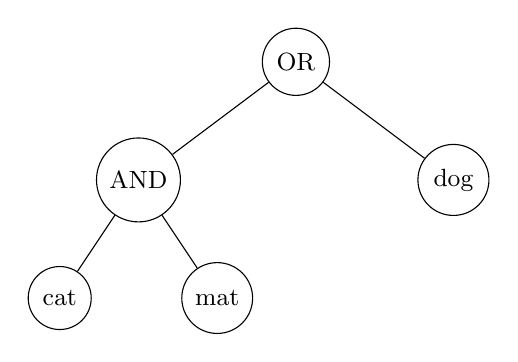
\begin{tikzpicture}[
    level distance=1.5cm,
    level 1/.style={sibling distance=4cm},
    level 2/.style={sibling distance=2cm},
    every node/.style={circle, draw, minimum size=0.8cm, font=\small}
]
    \node {OR}
        child {node {AND}
            child {node {cat}}
            child {node {mat}}
        }
        child {node {dog}};
\end{tikzpicture}
\end{document}
